\documentclass[11pt,a4paper]{article}
\usepackage[margin=22mm]{geometry}
\usepackage[T1]{fontenc}
\usepackage{lmodern}
\usepackage{graphicx,booktabs,tabularx,array,xcolor,enumitem,fancyhdr,hyperref}
\definecolor{reclaim}{HTML}{245D65}
\hypersetup{colorlinks=true,urlcolor=reclaim,linkcolor=reclaim}
\setlength{\parindent}{0pt}\setlength{\parskip}{5pt}
\setlist[enumerate]{nosep,leftmargin=18pt}
\pagestyle{fancy}\fancyhf{}
\fancyhead[L]{\textcolor{reclaim}{\textbf{RECLAIM}}}
\fancyhead[R]{Deliverable 1 | Track A}
\fancyfoot[L]{Artificial Intelligence Semester Project}\fancyfoot[R]{\thepage}
\setlength{\headheight}{14pt}
\newcommand{\smalltable}{\small\renewcommand{\arraystretch}{1.2}}
\begin{document}
{\LARGE\bfseries\color{reclaim} Reclaim}\\[3pt]
{\large Predicting return risk in e-commerce}\\[4pt]
\textbf{Deliverable 1: Problem Definition \& Data Foundations}\\
Track A: Application Development \hfill 24 October 2026
\begin{center}\smalltable
\begin{tabularx}{\linewidth}{Xll}
\toprule Team member & Student ID & GitHub\\ \midrule
Muhammad Soban Sohail & 24L-2545 & Soban06\\
Mahad Jawad Rana & 24L-2504 & Mahad-Jawad\\
Taimur Amir & 24L-2518 & taimurrrr\\ \bottomrule
\end{tabularx}\end{center}
\textbf{Repository:} \url{https://github.com/Soban06/Reclaim}
\section*{1. Problem definition}
Online retailers must handle uncertainty about which products will be returned. Returns create reverse-logistics, handling and inventory-planning work. Reclaim proposes a decision-support application that estimates return risk from product and customer context. The topic has been approved for Track A.

The intended users are e-commerce operations managers, inventory planners and customer experience staff. A future interface will accept purchase details, show a risk score and explain model signals. Scores should support planning and assistance rather than automatically refusing orders or return rights.

\subsection*{Prediction target and scope}
The initial dataset supports \textbf{purchase-event / product-variant return prediction}: \(y=1\) means returned and \(y=0\) means kept. It lacks order IDs connecting products into baskets. This phase therefore does not claim to predict the return of an entire multi-item order.

The intended prediction time is order placement. Only information available at that point should enter a deployed model. The original idea includes price, discount, customer history and shipping details. The release provides product-level averages and shipping country, not exact order prices, shipping methods or delivery dates. These distinctions guide feature selection.

\subsection*{Why machine learning?}
A fixed price-threshold rule cannot flexibly represent interactions between product type, brand and customer context. Supervised learning can estimate associations from labeled examples and produce a score evaluated on unseen data. Whether it improves upon simple rules remains an empirical question: majority-class and simple rule baselines will be compared with learned models in the next phase.

\subsection*{Current deliverable}
This submission implements documented acquisition, source verification, data-quality checks, joins, a reproducible sample, train-fitted preprocessing and exploratory analysis. Model training, prediction explanations and online deployment are future milestones. No predictive-performance result is claimed here.

\newpage
\section*{2. Data acquisition and provenance}
We selected the \textbf{ASOS GraphReturns} release from the original Open Science Framework repository [1], described by McGowan et al. [2]. It contains real, anonymized fashion-retail purchase outcomes, customer nodes and product-variant nodes. The paper describes training purchases from September--October 2021 and a later testing period. This deliverable uses the three \emph{training} files only.

OSF metadata identifies the license as \textbf{Creative Commons Attribution 4.0 International}. Attribution, source links and transformations are documented. Raw and processed datasets are excluded from Git; acquisition scripts and evidence are included.
\begin{center}\smalltable
\begin{tabularx}{\linewidth}{Xrr}
\toprule Original training table & Rows & Columns\\ \midrule
Purchase events & 1,369,133 & 3\\
Customers & 777,001 & 30\\
Product variants & 411,495 & 44\\ \bottomrule
\end{tabularx}\end{center}
The files total 364,102,152 bytes (about 364 MB). The downloader obtains the original file listing, checks SHA-256 hashes against OSF metadata, and records URLs, sizes and verification timestamps. The loader checks pinned hashes and restricts deserialization to required pandas/numpy object types.

\textbf{Evidence:} The original file listing, dataset/license metadata and timestamped download manifest are saved under \texttt{reports/evidence/}.
\begin{center}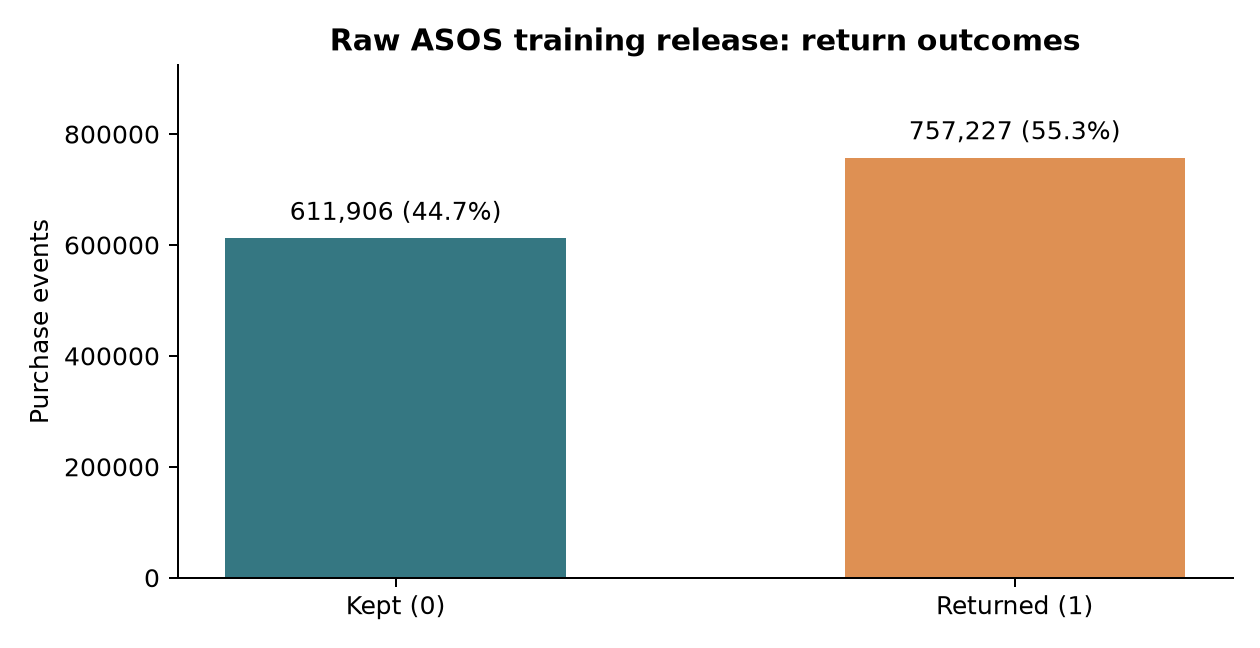
\includegraphics[width=.88\linewidth]{images/class_distribution.png}\end{center}
\textbf{Figure 1.} Raw outcomes: 611,906 kept and 757,227 returned events, or approximately 55.31\% returned. This is not the retailer's overall return rate.

\subsection*{Representativeness}
The paper states that included customers have at least one return, limiting generalization to customers without return history. Most category names are anonymized; \texttt{Country\_G}, for example, cannot be mapped to a real country. One historical fashion-retail sample does not represent all e-commerce domains. Official testing files remain unused in this phase.

\newpage
\section*{3. Cleaning and data-quality findings}
Every raw table is audited before sampling. No missing cells occur in the three files, but relational completeness is a separate issue.
\begin{center}\smalltable
\begin{tabularx}{\linewidth}{Xr}
\toprule Audit result & Count\\ \midrule
Repeated customer--variant--outcome tuples & 6,551\\
Events without a matching customer node & 71,648\\
Events without a matching product node & 474,590\\
Events missing either node (union) & 520,679\\
Events with both nodes available & 848,454\\
Complete events with implausible derived age & 12,099\\
Reproducible development sample & 100,000\\ \bottomrule
\end{tabularx}\end{center}
\textbf{Duplicates.} The implementation removes node-table exact duplicates before checking key uniqueness; none were found. Repeated event tuples are retained because no order ID or timestamp distinguishes duplicate records from legitimate repeat purchases. Both node tables repeat a return-reason column name; only explicitly selected, unambiguous fields enter the join.

\textbf{Joins.} Customer and product joins enforce many-to-one relationships. Events missing either node are excluded and counted. Missing-node counts overlap and must not be summed. Approximately 38.03\% of events are excluded; their return rate is 56.23\%. The exclusion can change the population and needs further investigation.

\textbf{Missing and invalid values.} Negative/nonfinite financial values and zero average prices become missing; none occur among complete events in this run. Approximate age uses the source year, 2021. Ages outside 0--100 become missing for auditing. Age and gender are excluded from predictors. The sampled age column has 1,413 missing values.

\textbf{Outliers.} Valid high prices remain in the cleaned data. Numerical preprocessing caps values at training-sample 1st and 99th percentiles, without learning bounds from validation rows or deleting high-value purchases.
\subsection*{Implemented data flow}
\begin{center}\fbox{\parbox{.91\linewidth}{\centering
OSF acquisition and checksum verification\\ \(\downarrow\)\\
Raw audit, explicit field selection and validated node joins\\ \(\downarrow\)\\
Complete events \(\rightarrow\) 100,000-event sample (seed 42)\\ \(\downarrow\)\\
Customer-group split \(\rightarrow\) train-fitted preprocessing\\ \(\downarrow\)\\
Sparse matrices, JSON evidence and exploratory figures}}\end{center}
The sample is not deliberately class-balanced. Its return fraction is 54.484\%.

\newpage
\section*{4. Feature strategy and preprocessing}
\begin{center}\smalltable
\begin{tabularx}{\linewidth}{p{.28\linewidth}X}
\toprule Field / group & Treatment and rationale\\ \midrule
Average product price & Median imputation, percentile clipping and standard scaling. Product-level GBP average, not exact order price.\\
Average discount & Same pipeline; retained in source units, not assumed to be a percentage or a GBP amount.\\
Product type, brand, shipping country & Most-frequent imputation and one-hot encoding; unknown categories ignored at transformation time.\\
Premier membership & Categorical membership indicator.\\
Customer and variant IDs & Join/split keys only, excluded from features.\\
Age and gender & Data-quality auditing only.\\
Sales/returns counts, return rates and reasons & Excluded because their timing relative to each target event is unverified.\\ \bottomrule
\end{tabularx}\end{center}
Standard scaling uses \(z=(x-\mu_{\mathrm{train}})/\sigma_{\mathrm{train}}\). Separate min--max normalization is unnecessary. One-hot encoding avoids an artificial category order.

A seeded customer-group split produces \textbf{80,000 training rows} and \textbf{20,000 validation rows}, with 75,588 and 18,897 distinct customers and \textbf{zero overlap}. All imputation, clipping, scaling and category fitting use training rows only. The sparse matrices contain 35 features.

Training/validation return rates are 54.54\%/54.25\%. Clipping bounds are GBP 4.16--100.32 for price and 12.86--21.27 for the source discount measure.

\textbf{Temporal limitation.} Customer grouping does not establish chronological validity. Product-average price and discount may include target-period information. Their timing must be verified or the fields replaced before production training. This is a preprocessing demonstration, not a leakage-free deployment benchmark.
\begin{center}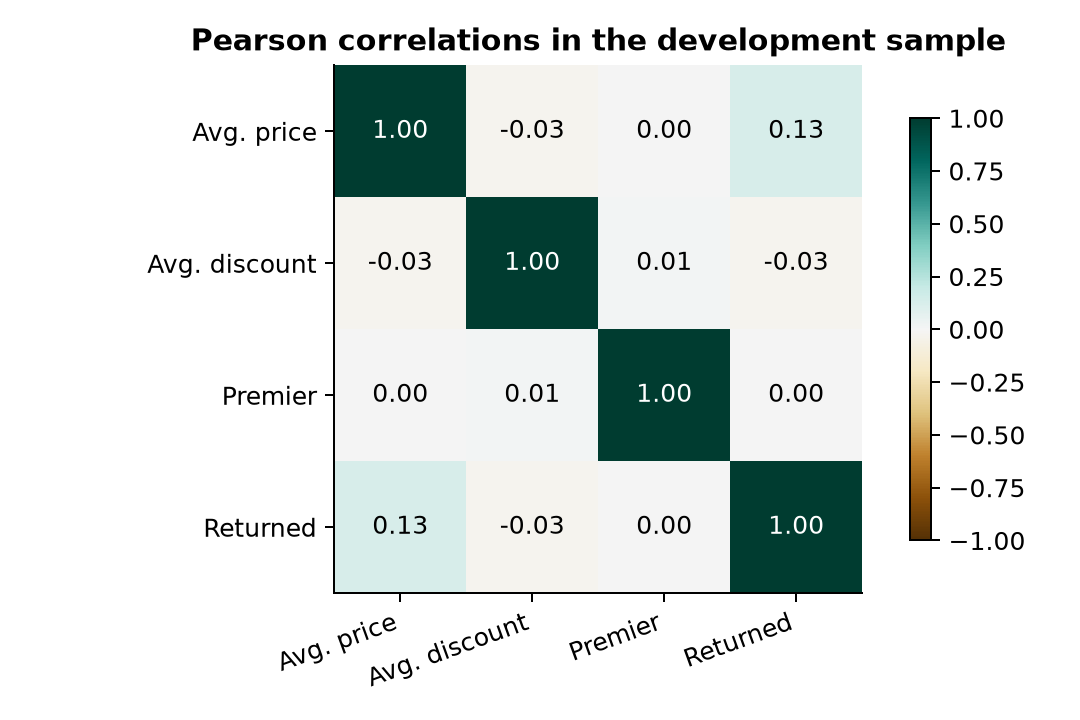
\includegraphics[width=.60\linewidth]{images/correlations.png}\end{center}
\textbf{Figure 2.} Price correlates modestly with return outcome (\(r=0.127\)); this is descriptive and does not establish causation.

\newpage
\section*{5. Initial exploratory analysis}
\begin{center}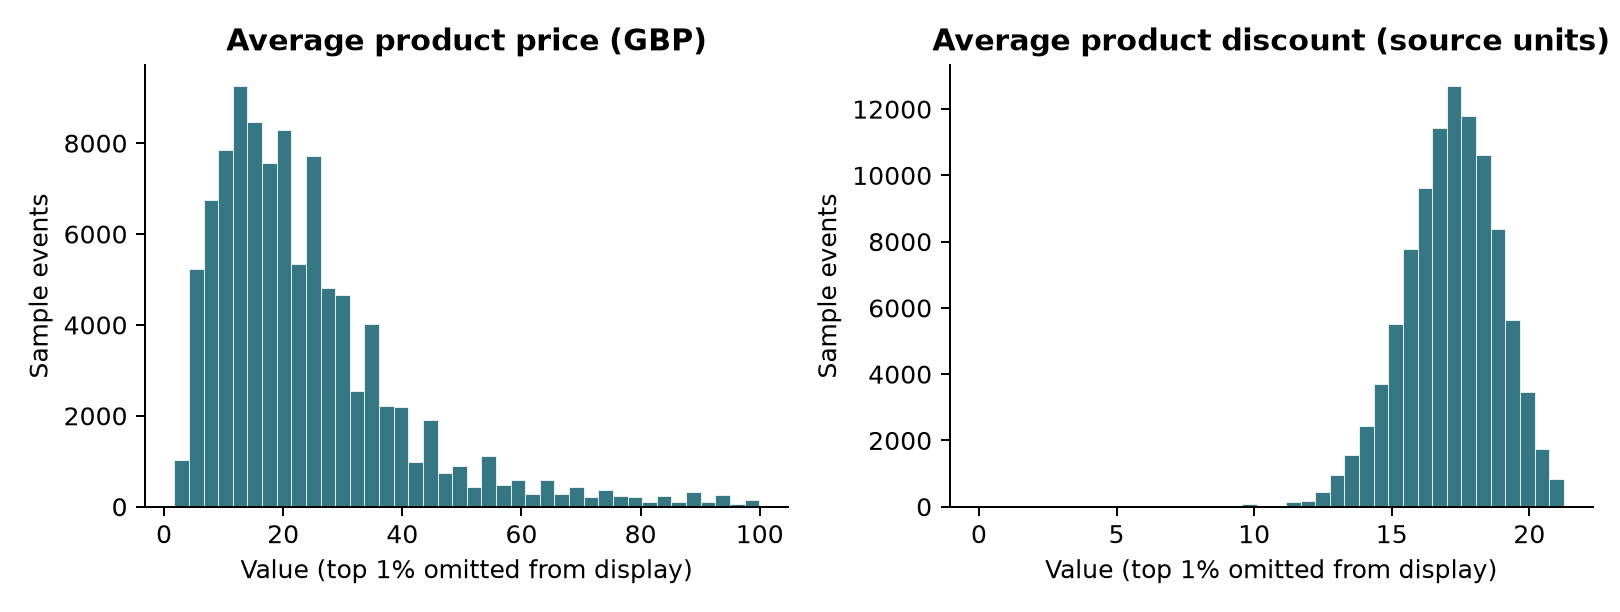
\includegraphics[width=\linewidth]{images/price_discount.png}\end{center}
\textbf{Figure 3.} Product-level averages across sampled events. The highest 1\% is omitted only from this visualization; those values remain in the cleaned sample.

Average price has a median of GBP 19.70, mean GBP 24.74 and maximum GBP 420.00. The larger mean is consistent with a right tail. Discount has a median of 17.26 in source units. These are event-weighted summaries of product averages, not order-level amounts.
\begin{center}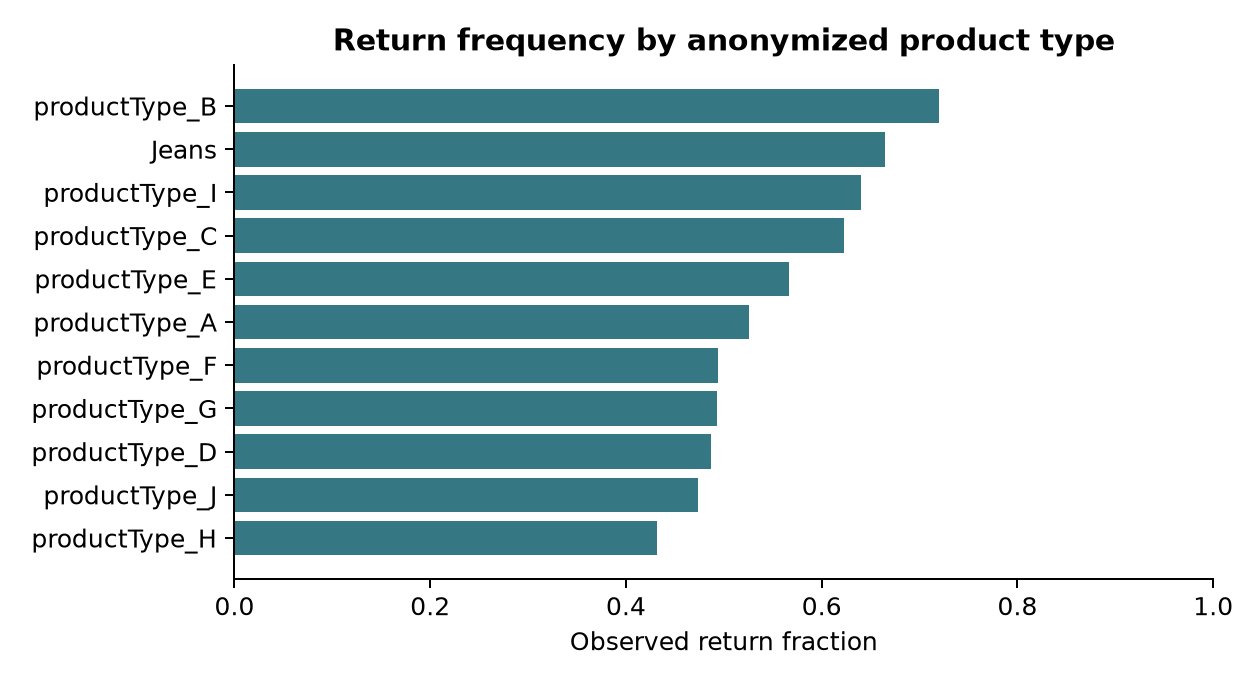
\includegraphics[width=.86\linewidth]{images/product_return_rates.png}\end{center}
\textbf{Figure 4.} Return frequency ranges from 43.18\% for \texttt{productType\_H} (\(n=7{,}819\)) to 72.01\% for \texttt{productType\_B} (\(n=16{,}294\)). The largest group, \texttt{productType\_J}, has 46,016 events and a 47.35\% return rate.

These differences motivate category-aware models, but are not evidence of predictive performance. Product mix, selection and missing-node exclusions may contribute. The weak discount correlation (\(r=-0.029\)) does not establish that it is useless; interactions may exist.

\newpage
\section*{6. Bias checks, limitations and next phase}
\begin{center}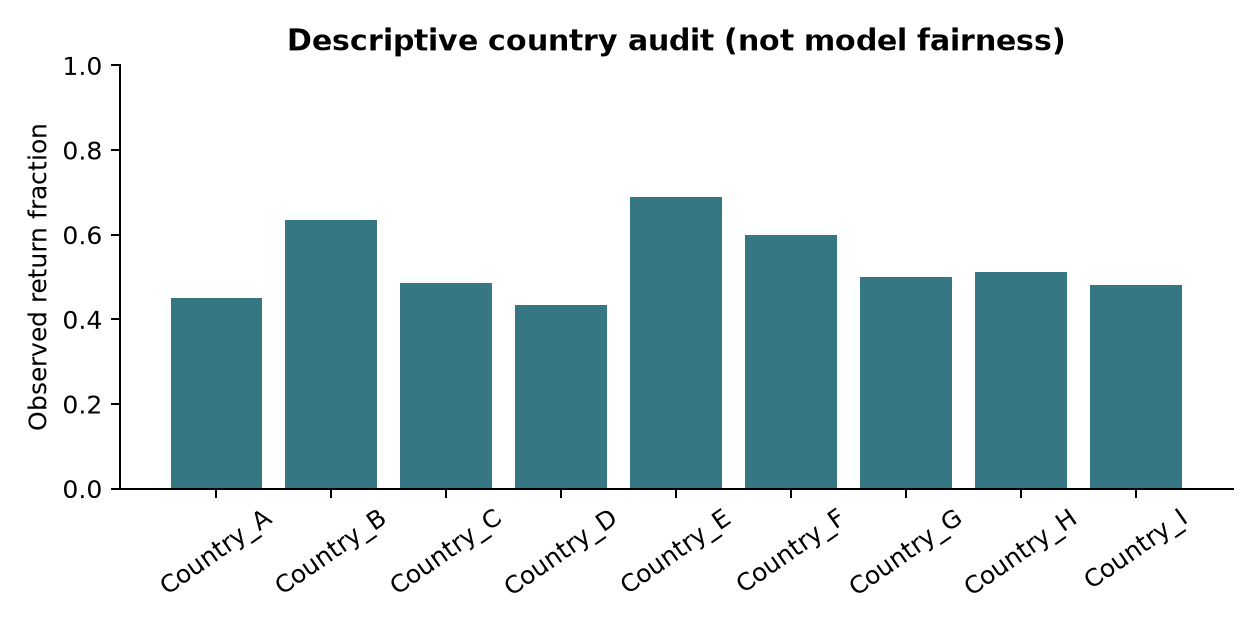
\includegraphics[width=.78\linewidth]{images/country_audit.png}\end{center}
\textbf{Figure 5.} Country return fractions range from 43.43\% to 68.79\%. Country\_G accounts for 55,392 sample events, while several groups have fewer than 2,000.

This is a dataset-level check, not proof of model fairness. Later evaluation should compare precision, recall, false-positive rates and calibration across sufficiently supported groups. Omitting demographics does not remove all bias because other features may act as proxies.

\textbf{Limitations.} Selection on return history, missing node matches, anonymized labels, uncertain aggregate timing and absent order baskets/dates constrain the work. No official test-period evaluation, calibrated probability or business-savings claim is made.
\subsection*{Planned Track A implementation}
\begin{enumerate}
\item Resolve aggregate timing and missing-node provenance; assess a later-period test.
\item Compare majority/rule baselines, logistic regression and a tree classifier. Report precision, recall, F1, PR-AUC, ROC-AUC, confusion matrices and calibration.
\item Choose thresholds on validation data using explicit false-alarm/missed-return costs.
\item Host the interface and backend, reusing the fitted preprocessing pipeline.
\end{enumerate}
\subsection*{Team workflow}
Proposed responsibilities: Soban handles problem definition, report integration and coordination; Mahad handles acquisition, provenance and cleaning; Taimur handles preprocessing, EDA and validation. Each reviews and runs their part and commits under their own account. This is a work allocation, not a claim that all reviews and commits have occurred.

Generative AI assisted with drafting and implementation. Members remain responsible for understanding and validating the work. The README gives the execution sequence; JSON evidence and chart scripts make results inspectable.
\small
\begin{thebibliography}{9}
\bibitem{data} ASOS. \emph{ASOS graph returns dataset}. OSF, 2022. \url{https://osf.io/c793h/}. CC BY 4.0. Accessed 24 October 2026.
\bibitem{paper} J. McGowan et al. \emph{A Dataset for Learning Graph Representations to Predict Customer Returns in Fashion Retail}. 2023. \url{https://arxiv.org/abs/2302.14096}.
\end{thebibliography}
\end{document}
